\documentclass[11pt]{article}
\usepackage{amsmath}
% use UTF8 encoding
\usepackage[utf8]{inputenc}
% use KoTeX package for Korean
\usepackage{kotex}

\usepackage{hyperref}

\usepackage{graphicx}

\hypersetup{
    colorlinks=true,   
    urlcolor=red,
}

\title{머신러닝}

\author{Minwoo Jung}

\begin{document}

\maketitle

\section{CNN}

\subsection{전체구조}

\indent \\합성곱 신경망(CNN)은 이미지 및 음성을 인식할 수 있는 가장 기본 딥러닝 기법이다. 인접하는 계층의 모든 뉴런과 결합되어 있는 상태를 완전연결(Fully connected)이라고 정의하며, 완전히 연결된 계층을 Affine 계층이라고 부른다. Affine 변환은 기하학에서 행렬의 곱을 부르는 이름이다. 
	\begin{figure}
		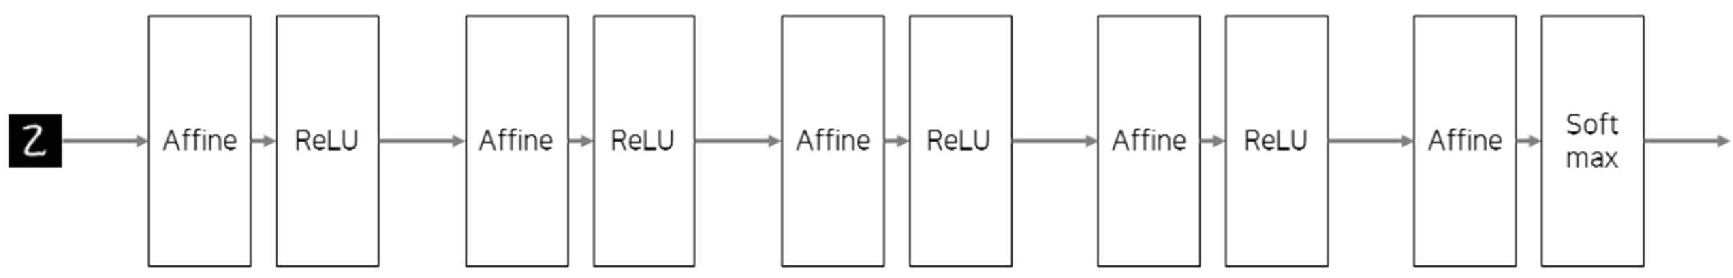
\includegraphics[width=1\columnwidth]{../Figure/Figure_1.pdf}
	\end{figure}
    \begin{figure}
		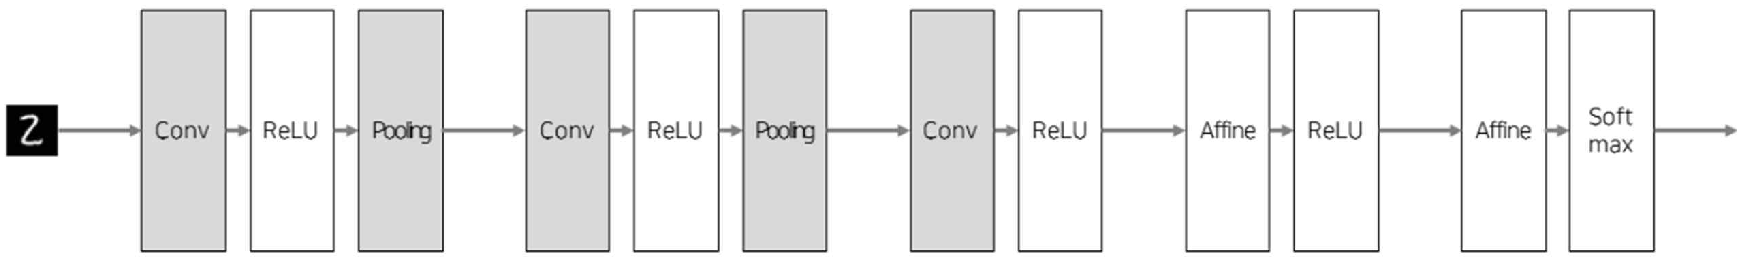
\includegraphics[width=1\columnwidth]{../Figure/Figure_2.pdf}
	\end{figure}	
\indent \\'Affine-ReLU' 연결이 CNN 계층으로 바뀌면서 'Conv-ReLU-(Pooling)'으로 바뀌었다.

\subsection{합성곱계층}

\subsubsection{완전연결 계층의 문제점}
\indent \\완전연결의 문제점은 데이터 형상이 무시된다. 특징맵, 합성곱연산, 필터=>커널, 패딩, 스트라이드(필터를 적용하는 위치의 간격),
\subsubsection{합성곱 연산}
\subsubsection{패딩}
\subsubsection{스트라이드}
\subsubsection{3차원 데이터의 합성곱 연산}
\subsubsection{블록으로 생각하기}
\subsubsection{배치처리}
\subsection{풀링계층}


$$ OH = \dfrac{H+2P-FH}{S} + 1 \\

$$ OW = \dfrac{W+2P-FW}{S} + 1 \\


\end{document}
